\chapter{Teoría de grafos}
\addcontentsline{toc}{chapter}{Teoría de grafos}

En el ámbito de las matemáticas y las ciencias de la computación, se emplea el término \emph{grafo} (del griego \emph{grafos} que significa \emph{dibujo} o \emph{imagen}) para referirse a un conjunto de objetos llamados \emph{vértices} o \emph{nodos}, los cuales están unidos por enlaces conocidos como \emph{aristas} o \emph{arcos}. Estas conexiones representan las relaciones binarias que existen entre los elementos de un conjunto, y son objeto de estudio de la teoría de grafos.

\section{Grafos}

\begin{wrapfigure}{r}{0.4\textwidth}
\centering
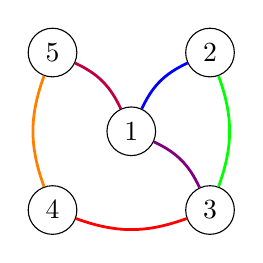
\begin{tikzpicture}

% Posiciones fijas de los nodos
\node[circle, draw=black, fill=white] (1) at (0,0) {1};
\node[circle, draw=black, fill=white] (2) at (1,1) {2};
\node[circle, draw=black, fill=white] (3) at (1,-1) {3};
\node[circle, draw=black, fill=white] (4) at (-1,-1) {4};
\node[circle, draw=black, fill=white] (5) at (-1,1) {5};

% Arcos aleatorios
\draw[-, blue, line width=1pt] (1) to[bend left=20] (2);
\draw[-, green, line width=1pt] (2) to[bend left=20] (3);
\draw[-, red, line width=1pt] (3) to[bend left=20] (4);
\draw[-, orange, line width=1pt] (4) to[bend left=20] (5);
\draw[-, purple, line width=1pt] (5) to[bend left=20] (1);
\draw[-, violet, line width=1pt] (1) to[bend left=20] (3);

\end{tikzpicture}
\caption{Ejemplo de grafo simple.}
\label{fig:grafo1}
\end{wrapfigure}

En esta sección se introducirán las deficiones básicas que forman parte de la teoría de grafos.

\begin{definition}
Matemáticamente, un \emph{grafo} $G = (V,E)$ es una tupla de vértices $V$ y aristas $E$ que relacionan dichos vértices. Denominaremos  \emph{orden} del grafo al número de vértices del mismo ($|V|$). Por supuesto, siempre tendremos que $V \neq \emptyset$.
\end{definition}

\begin{exampleth}
El grafo dado en la Figura \ref{fig:grafo1} tiene conjunto de vértices $V=\left\lbrace 1,2,3,4,5 \right\rbrace$ y conjunto de aristas $E=\left\lbrace (1,2),(1,3),(2,3),(3,4),(4,5),(5,1) \right\rbrace$.
\end{exampleth}

\begin{definition}
Un \emph{vértice} o \emph{nodo} es la unidad fundamental de las que se componen los grafos. Los vértices en sí mismos se tratan como objetos indivisibles y sin propiedades. No obstante, pueden tener asociados una semántica dependiendo del contexto de aplicación del grafo. Por ejemplo, en el grafo \ref{fig:DBA1516P2GA2} un nodo representa la consecución de un objetivo de un problema.
\end{definition}

\begin{definition}
Una \emph{arista} representa una relación entre dos vértices de un grafo. Las aristas se denotan por $(u,v) \in E$ donde $u,v\in V$. Visualmente, se representan como las líneas que unen los vértices que forman parte de la definición de la misma.
\end{definition}

\begin{definition}
Un \emph{grafo podenderado} es un grafo cuyas aristas tienen un peso o valor asociado.

Formalmente, se puede definir como un trío ordenado $G=(V,E,W)$ donde $V=\left\lbrace v_1, \dots, v_n \right\rbrace$ es un conjunto de vértices, $E = \left\lbrace e_1, \dots, e_m \right\rbrace$ y $W = \left\lbrace w_1,\dots,w_m\right\rbrace$ es el conjunto de pesos asociados a cada arista.
\end{definition}

\deactivatequoting
\begin{figure}[H]
  \centering
\begin{minipage}[t]{0.45\linewidth}
\centering
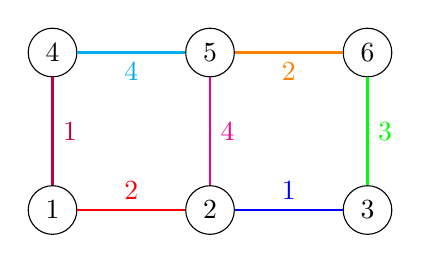
\begin{tikzpicture}
  \node[circle, draw] (1) at (0,0) {1};
  \node[circle, draw] (2) at (2,0) {2};
  \node[circle, draw] (3) at (4,0) {3};
  \node[circle, draw] (4) at (0,2) {4};
  \node[circle, draw] (5) at (2,2) {5};
  \node[circle, draw] (6) at (4,2) {6};

  \draw[red, line width=1pt] (1) -- node[midway, above] {2} (2);
  \draw[blue, line width=1pt] (2) -- node[midway, above] {1} (3);
  \draw[green, line width=1pt] (3) -- node[midway, right] {3} (6);
  \draw[cyan, line width=1pt] (4) -- node[midway, below] {4} (5);
  \draw[orange, line width=1pt] (5) -- node[midway, below] {2} (6);
  \draw[purple, line width=1pt] (4) -- node[midway, right] {1} (1);
  \draw[magenta, line width=1pt] (2) -- node[midway, right] {4} (5);
\end{tikzpicture}
\caption{Ejemplo de grafo ponderado.}
\label{fig:grafo2}
\end{minipage}
\hspace{0.5cm}
\begin{minipage}[t]{0.45\linewidth}
\centering
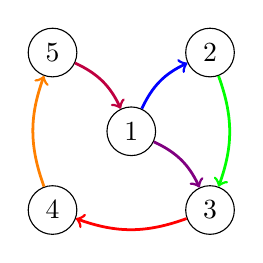
\begin{tikzpicture}

% Posiciones fijas de los nodos
\node[circle, draw=black, fill=white] (1) at (0,0) {1};
\node[circle, draw=black, fill=white] (2) at (1,1) {2};
\node[circle, draw=black, fill=white] (3) at (1,-1) {3};
\node[circle, draw=black, fill=white] (4) at (-1,-1) {4};
\node[circle, draw=black, fill=white] (5) at (-1,1) {5};

% Arcos aleatorios
\draw[->, blue, line width=1pt] (1) to[bend left=20] (2);
\draw[->, green, line width=1pt] (2) to[bend left=20] (3);
\draw[->, red, line width=1pt] (3) to[bend left=20] (4);
\draw[->, orange, line width=1pt] (4) to[bend left=20] (5);
\draw[->, purple, line width=1pt] (5) to[bend left=20] (1);
\draw[->, violet, line width=1pt] (1) to[bend left=20] (3);

\end{tikzpicture}
\caption{Ejemplo de grafo dirigido.}
\label{fig:grafo3}
\end{minipage}
\end{figure}
\activatequoting

\begin{definition}
Un \emph{grafo no dirigido} es un grafo cuyas aristas representan relaciones simétricas y  carecen de sentido definido. Es decir, la arista $(u,v)$ es idéntica a la arista $(v,u)$. Es decir, las aristas no son pares ordenados sino conjuntos $\left\lbrace u,v \right\rbrace$ (o $2$-multiconjuntos) de vértices.

Un grafo no dirigido podrá tener, a lo más, $\frac{|V|^2}{2}$ aristas.
\end{definition}

\begin{definition}
Se denomina \emph{grafo dirigido} o \emph{digrafo} a aquellos grafos cuyas aristas tengan un sentido definido. En un digrafo, cada arista se representa como un par ordenado de dos vértices. Por ejemplo, $(u,v)$ denota la arista que va de $u$ hacia $v$ (desde el primer vértice hasta el segundo vértice).

Los grafos no dirigidos se pueden ver como un caso particular de los grafos dirigidos en tanto que son grafos dirigidos simétricos.

Mientras que en un grafo no dirigido se tiene que $E \subseteq \{x \in \mathcal{P}(V) : |x| = 2\}$ (es decir, $E$ es un conjunto de pares no ordenados de elementos de $V$), cuando el grafo es dirigido se tiene que $E$ es un conjunto de pares ordenados $(i,j) \in V \times V$.
\end{definition}

\begin{exampleth}
En la Figura \ref{fig:grafo3} se muestra un ejemplo de grafo dirigido mientras que en la Figura \ref{fig:grafo1} tenemos un ejemplo de grafo no dirigido.
\end{exampleth}

\begin{wrapfigure}{r}{0.4\textwidth} %this figure will be at the right
    \centering
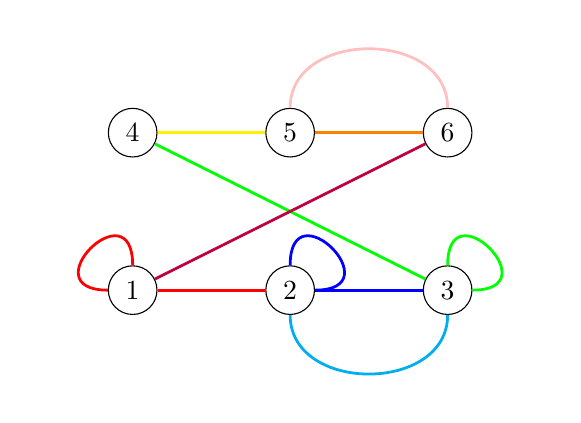
\begin{tikzpicture}
  \node[circle, draw] (1) at (0,0) {1};
  \node[circle, draw] (2) at (2,0) {2};
  \node[circle, draw] (3) at (4,0) {3};
  \node[circle, draw] (4) at (0,2) {4};
  \node[circle, draw] (5) at (2,2) {5};
  \node[circle, draw] (6) at (4,2) {6};

  \draw[red, line width=1pt] (1) -- (2);
  \draw[blue, line width=1pt] (2) -- (3);
  \draw[green, line width=1pt] (3) -- (4);
  \draw[yellow, line width=1pt] (4) -- (5);
  \draw[orange, line width=1pt] (5) -- (6);
  \draw[purple, line width=1pt] (6) -- (1);

  \draw[red, line width=1pt] (1) to [out=90, in=180, loop, distance=1cm] (1);
  \draw[blue, line width=1pt] (2) to [out=90, in=0, loop, distance=1cm] (2);
  \draw[green, line width=1pt] (3) to [out=90, in=0, loop, distance=1cm] (3);
  \draw[pink, line width=1pt] (5) to [out=90, in=90, loop, distance=1cm] (6);
  \draw[cyan, line width=1pt] (2) to [out=270, in=270, loop, distance=1cm] (3);
\end{tikzpicture}
	\caption{Ejemplo de multigrafo.}
	\label{fig:grafo4}
\end{wrapfigure}

\begin{definition}
Un \emph{grafo conexo} es un grafo en que todos sus vértices están conectados por un camino o por un semicamino dependiendo de si el grafo es no dirigido o dirigido.

De lo contrairo, si algún grafo no cumple la propiedad anterior se dirá que es \emph{disconexo}.
\end{definition}

\begin{definition}
Un \emph{bucle} es una arista que relacionado un vértice consigo mismo.
\end{definition}

\begin{definition}
En un grafo $G=(V,E)$, se dice que dos aristas son \emph{paralelas} o \emph{múltiples} si el vértice inicial y el vértice final de las mismas coinciden. 

Los grafos que permiten la existencia de bucles y aristas múltiples se denominan \emph{multigrafos}. Por el contrario, los grafos sin bucles y sin aristas paralelas se denominarán \emph{simples}.
\end{definition}

\begin{exampleth}
En la Figura \ref{fig:grafo2} tenemos un ejemplo de grafo ponderado.

En la Figura \ref{fig:grafo1} se muestra un ejemplo de grafo simple. Por otro lado, en la Figura \ref{fig:grafo4} podemos ver un multigrafo.
\end{exampleth}

\begin{definition}
En un grafo $G=(V,E)$ dos vértices se dirán \emph{adyacentes} (o \emph{vecinos}) si están relacionados por al menos una arista. Es decir, dos vértices $u,v \in V$ son adjacentes si $\exists e \in E$ tal que $e = (u,v)$.

La \emph{matriz de adyacencia} de un grafo es una matriz cuadrada de dimensión $|V| \times |V|$ que se utiliza como forma de representar las relaciones binarias entre los nodos del mismo. La denotaremos por $A = (a_{ij})_{1\leq i,j\leq |V|}$.

Si tenemos que $G$ es un grafo no dirigido, entonces $a_{ij} = 1$ y $a_{ji} = 1$ si el vértice $v_i$ es adyacente al vértice $v_j$ y $a_{ij} = a_{ji} = 0$ en caso contrario. Si el grafo $G$ es dirigido, entonces tendremos que $a_{ij} = 1$ si y sólo si existe $e \in E$ tal que $e = (v_i,v_j)$ y $a_{ij} = 0$ en caso contrario.

Por último, si tenemos un grafo ponderando, entonces se sustiuirá en valor de $1$ en los casos anteriores por el peso de las aristas correspondientes.
\end{definition}

\begin{exampleth}
Tenemos que la matriz de adyacencia del grafo de la Figura \ref{fig:grafo1} es:
\begin{equation}
\begin{pmatrix}
0 & 1 & 1 & 0 & 1\\
1 & 0 & 1 & 0 & 0\\
1 & 1 & 0 & 1 & 0\\
0 & 0 & 1 & 0 & 1\\
1 & 0 & 0 & 1 & 0
\end{pmatrix}
\end{equation}
\end{exampleth}

\begin{definition}
Sea $G=(V,E)$ un grafo no dirigido y sea $v \in V$ un vértice suyo. Se denomina grado del vértice $v$ al número de aristas incidentes al vértice y se denotará de ahora en adelante por $\text{deg}(v)$.

Al conjunto de todos los vértices adyacentes a un vértice dado se le denominará \emph{vecindad} del vértice en cuestión. Formalmente, la vecindad de un vértice $v \in V$ es el conjunto
\begin{equation}
N(v) = \left\lbrace u \in V | \left\lbrace v,u\right\rbrace \in E \right\rbrace
\end{equation}

Así pues, el grado de un vértice $v \in V$ puede definirse como el módulo de su vecindario: $\text{deg}(v) = |N(v)|$.

En el caso de los grafos dirigidos se distingue entre el \emph{grado de entrada} $\text{deg}^-(v)$ (número de aristas que tienen a $v$ como el vértice final) y el \emph{grado de salida} $\text{deg}^+(v)$ (número de ariastas que tienen a $v$ como vértice inicial). 
\end{definition}

% Meter Lema del apetrón de manos?

\begin{wrapfigure}{r}{0.4\textwidth}
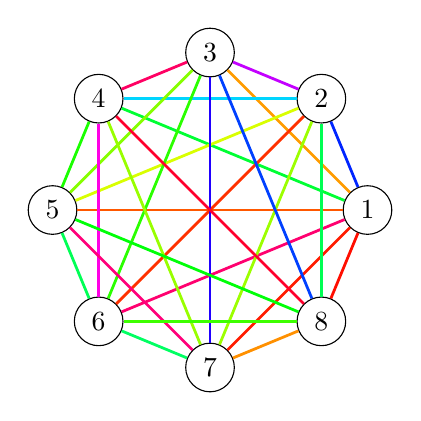
\begin{tikzpicture}
  \foreach \x in {1,...,8}{
    \node[circle, draw] (\x) at ({45*(\x-1)}:2) {\x};
  }

  \foreach \x in {1,...,7}{
    \foreach \y in {\x,...,8}{
      \pgfmathsetmacro\randhue{rnd}
      \definecolor{mycolor}{hsb}{\randhue, 1, 1}
      \draw[mycolor, line width=1pt] (\x) -- (\y);
    }
  }
\end{tikzpicture}
\caption{Ejemplo de grafo completo.}
	\label{fig:grafo5}
\end{wrapfigure}

\begin{definition}
Un grafo en el que todos sus vértices tienen el mismo grado (de entrada, en el caso de los grafos dirigidos) se denomina \emph{regular}. Además, un grafo con vértices de grado $k$ se llamará $k$-regular.
\end{definition}

\begin{definition}
Un \emph{grafo completo} $G=(V,E)$ es un grafo no dirigido simple en el que para cada par de vértices $u, v\in V$ existe una arista $e \in E$ tal que $e = \left\lbrace u,v\right\rbrace$.

El \emph{grafo completo de $n$ vértices} se denotará por $K_n$. Así pues, $K_n$ tendrá $frac{n\cdot (n-1)}{2}$ aristas y es un grafo regular de grado $n-1$.
\end{definition}

\begin{figure}[H]
  \centering
\begin{minipage}[t]{0.45\linewidth}
\centering
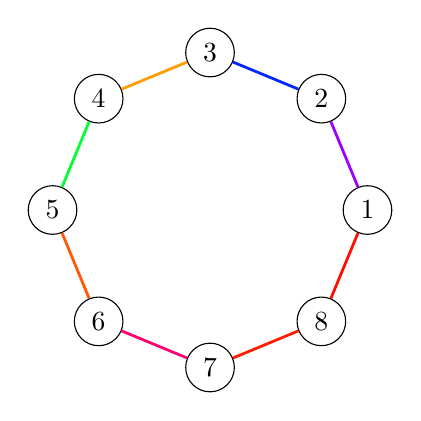
\begin{tikzpicture}
  \foreach \x in {1,...,8}{
    \node[circle, draw] (\x) at ({45*(\x-1)}:2) {\x};
  }

  \foreach \x in {1,...,7}{
      \pgfmathsetmacro\randhue{rnd}
      \definecolor{mycolor}{hsb}{\randhue, 1, 1}
      \pgfmathtruncatemacro{\next}{\x + 1}
      \draw[mycolor, line width=1pt] (\x) -- (\next);
  }
  \pgfmathsetmacro\randhue{rnd}
  \definecolor{mycolor}{hsb}{\randhue, 1, 1}
  \draw[mycolor, line width=1pt] (8) -- (1);
\end{tikzpicture}
\caption{Ejemplo de grafo ciclo.}
	\label{fig:grafo6}
\end{minipage}
\hspace{0.5cm}
\begin{minipage}[t]{0.45\linewidth}
\centering
    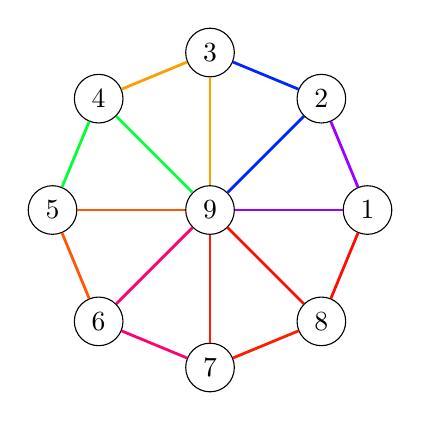
\begin{tikzpicture}
  \foreach \x in {1,...,8}{
    \node[circle, draw] (\x) at ({45*(\x-1)}:2) {\x};
  }
  \node[circle, draw] (9) at (0,0) {9};

  \foreach \x in {1,...,7}{
      \pgfmathsetmacro\randhue{rnd}
      \definecolor{mycolor}{hsb}{\randhue, 1, 1}
      \pgfmathtruncatemacro{\next}{\x + 1}
      \draw[mycolor, line width=1pt] (\x) -- (\next);
      \draw[mycolor, line width=1pt] (\x) -- (9);
  }
  \pgfmathsetmacro\randhue{rnd}
  \definecolor{mycolor}{hsb}{\randhue, 1, 1}
  \draw[mycolor, line width=1pt] (8) -- (1);
  \draw[mycolor, line width=1pt] (8) -- (9);
\end{tikzpicture}
\caption{Ejemplo de grafo rueda.}
\label{fig:grafo7}
\end{minipage}
\end{figure}

\begin{definition}
Un \emph{grafo ciclo} o simplemente un \emph{ciclo} es un grafo que consiste en un camino simple cerrado. Esto es, hay un único camino en el que no se repite ningún vértice salvo el primero con el último.

Denotaremos a un grafo ciclo de $n$ vértices por $C_n$. Si consideramos que es un grafo no dirigido, cada vértice tendrá un vecindario de tamaño $2$ y, por tanto, será un grafo $2$-regular. Por el contrario, si tenemos un grafo dirigido, será un grafo $1$-regular.
\end{definition}

\begin{definition}
Un grafo rueda es un grafo de $n$ vértices (denotado usualmente por $W_n$) es un grafo que se obtiene al añadir un único vértice a un grafo ciclo de $n-1$ vértices, conectando el nuevo el vértice a todos los ya existentes. Es decir, el nuevo vértice será adyacente a todos los vértices del grafo $C_{n-1}$.
\end{definition}

\begin{exampleth}
En las Figuras \ref{fig:grafo5}, \ref{fig:grafo6} y \ref{fig:grafo7} podemos ver un grafo completo, un grado ciclo y un grafo rueda respectivamente.
\end{exampleth}

\begin{definition}
Diremos que un grafo es \emph{cíclico} si contiene al menos un grafo ciclo. Por el contrario, se dirá que un grafo es \emph{acíclico} si no contiene ningún ciclo.

No obstante, en este trabajo fin de grado nos centraremos en los llamados \emph{grafos dirigidos acíclicos} o \emph{DAG} (\emph{Directed Acyclic Graphs}, en inglés) que no son más que grafos dirigidos desprovistos de ciclos.
\end{definition}

\begin{wrapfigure}{l}{0.4\textwidth}
\centering
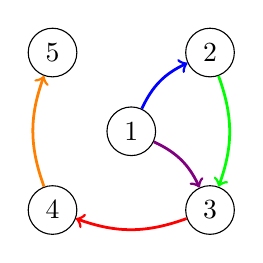
\begin{tikzpicture}

% Posiciones fijas de los nodos
\node[circle, draw=black, fill=white] (1) at (0,0) {1};
\node[circle, draw=black, fill=white] (2) at (1,1) {2};
\node[circle, draw=black, fill=white] (3) at (1,-1) {3};
\node[circle, draw=black, fill=white] (4) at (-1,-1) {4};
\node[circle, draw=black, fill=white] (5) at (-1,1) {5};

% Arcos aleatorios
\draw[->, blue, line width=1pt] (1) to[bend left=20] (2);
\draw[->, green, line width=1pt] (2) to[bend left=20] (3);
\draw[->, red, line width=1pt] (3) to[bend left=20] (4);
\draw[->, orange, line width=1pt] (4) to[bend left=20] (5);
\draw[->, violet, line width=1pt] (1) to[bend left=20] (3);

\end{tikzpicture}
\caption{Ejemplo de grafo acíclico dirigido con $5$ nodos.}
\label{fig:grafo8}
\end{wrapfigure}

\begin{exampleth}
En la Figura \ref{fig:grafo1} tenemos un grafo dirigido con ciclos o cíclico (contiene, por ejemplo, el $1$-$3$-$4$-$5$). Sin embargo, eliminado una de las aristas del mismo obtenemos el grafo de la Figura \ref{fig:grafo8}, que es acíclico. 
\end{exampleth}

\begin{definition}
Un grafo conexo acíclico no dirigido se denominará \emph{árbol}. Por otro lado, un \emph{árbol orientado} o \emph{poliárbol} será un grafo dirigido acíclico cuyo grafo no dirigido subyacente es un árbol. De otra manera, si cambiamos sus aristas dirigidas por no diridas, se obtendía un grafo no dirigido conexo y acíclico.
\end{definition}

\begin{definition}
Un \emph{árbol de expansión} de un grafo conexo no dirigido $G$ es un subgrafo suyo que es árbol y que contiene a todos sus vértices.

El \emph{número de árboles de expansión} de un grafo conexo $G$, habitualmente denotado por $t(G)$, es un invariante importante en la teoría de grafos. Éste puede obtenerse mediante el denominado \emph{Teorema de Kirchhoff}. Este teorema demuestra que el número de árboles de expansión de un grafo puede obtenerse en tiempo polinómico a partir del determinante de una submatriz de la \emph{matriz Laplaciana} del grafo. Más aún, nos dice que éste número es igual a cualquier cofactor de la matriz Laplaciana. El Teorema de Kirchhoff es una generalización de la \emph{fórmula de Cayley}, que proporciona el número de árboles de expansión en el caso de un grafo completo y que veremos a continuación.
\end{definition}

\begin{proposition}
Dado un grafo completo $K_n$, la fórmula de Cayley establece que el número de árboles de expansión del mismo es $t(K_n) = n^{n-2}$.
\end{proposition}